% B.tex (for normal text)
\section{VK}
Vk.com is the most popular social network in Russia. Today vk has about 400 millions accounts. 80 millions visitors come to the site every day. 
\subsection{Getting data from vk}
Vk.com provide grat api for developers. API interface allows information to be received from the database vk.com with the help of http-requests to the special server. We do not need to know in detail how the base is constructed and from which table and field types it consists of. It is enough that API-request “knows” it. The request syntax and the type of data being returned are strictly determined by the service itself. 
For example, to receive data about the user with the ID number “210700286”, you need to make a request of this type:


\begin{lstlisting}
	https://api.vk.com/method/users.get?user_ids=396547478&fields=online,last_seen&v=5.60
\end{lstlisting}

Let’s have a look at the individual parts:
\begin{itemize}
	\item{\texttt{api.vk.com/methods} — API server address}
	\item{\texttt{users.get} — name of API VKontakte’s “method”. Methods represent conditional commands that correspond with an operation from the database to receive, record or delete information. For example, users.get is a method to receive information about a user.}
	\item{\texttt{user{\_}ids=396547478{\&}fields=online,last{\_}seen{\&}v=5.60}  – parameter request.}
\end{itemize}
	
In its response, the server returns JSON-object with the requested data (or a message about a mistake if something went wrong). 

The response to our request looks like this:
\begin{lstlisting}
	{"response":[{"id":396547478,"first_name":"Ssn","last_name":"Project","online":0,"last_seen":{"time":1480705322,"platform":7}}]}
\end{lstlisting}

Let’s have a close look at fields that is interesting for us:
\begin{itemize}
	\item{online information whether the user is online.  Returned values: 1 — online, 0 — offline.  If user utilizes a mobile application or site mobile version, it returns online{\_}mobile additional field that includes 1. With that, in case of application, online{\_}app additional field is returned with application ID.}  
	\item{last{\_}seen	last visit date.  Returns last{\_}seen object with the following fields:
	\begin{itemize}
		\item{time - last visit date (in Unix time).}
		\item{platform - type of the platform that used for the last authorization.}
	\end{itemize}}
\end{itemize}

In this paper we will use only two methods: users.get which returns detailed information on users and wall.get which returns a list of posts on a user wall or community wall.


\subsection{Find ip range of vk}
Vk.com has two ip range 87.240.128.0/18 and 95.213.0.0/18. To figure it out we first ping vk.com, when we take given ip and check information about it by using utility whois it give use we network mask for this ip. Also we check that vk.com dose not have any another ip by using utility dig and check that id don't return any another ip addresses.


\subsection{Experimental results}
For the experiments we created test profile https://vk.com/id396547478 and fill wall with some text posts in different time and day. For netflow collection we will use nfdump[????????????], and for real test we will use real netflow traffic from university Innopolis. 
\subsubsection{Matching IP to profile by analyzing wall posts}
Wall post can be different format(music, video, link, repost, photo, text message), the text message posts is the popular and the hard one, because it is very similar to personal text message that people send to each other every second. So you can not see difference between them in the netflow traffic. We are lucky if a user posts photo, it is have 3 fields that we can analyze: post publish time, photo upload time, photo size. But we will look only at difficult case when all post it is small text message similar to the message that users exchange in dialogs. If we able match ip in this case we will able do it in easier case, because text message posts has only one field for analysis:post publish time. For this purpose was written program in python language that take last n post, get timestamp from it and for each timestamp it crate list with all unique ip that do request to vk in this second(+-1s) Then it print IPs that was spotted in each list. In figure [1?????????] you can see we correlation between matched IP and number of post. 
 
\begin{figure}[H]%\label{wall}   [\ref{wall}]
	\centering{
		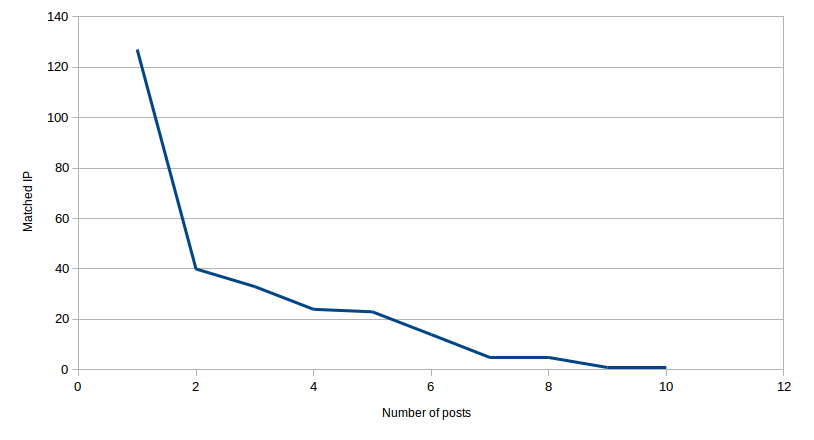
\includegraphics[width=180mm]{images/vk/wall.png}
		\caption{correlation between matched IP and number of post}
	}
\end{figure}

\subsubsection{Problems}
The main problem we did not know that the user post posts from the same ip, only that we can know it was or PC or mobile app. 

The second main problem that we have to many active user in the same time, as you can see fome figure [2????????] in pick time we have about 350 unique ip do request to vk server. 

The third problem it can be less then 9 post with the same IP addresses(from diagram [1?????????] we saw that we need more then 9 post to match IP).
Solutions for this problems will be consider in next section.
\begin{figure}
	\centering{
		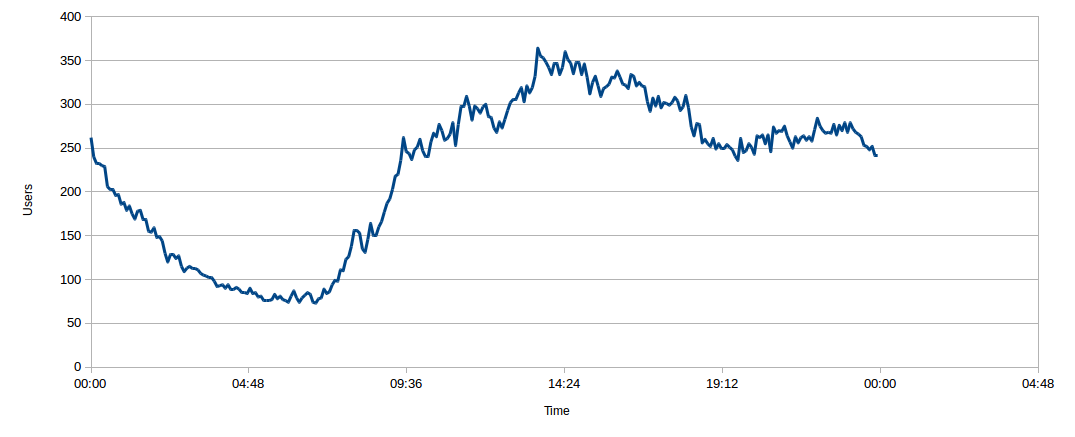
\includegraphics[width=180mm]{images/vk/users.png}
		\caption{Number of vk active users in UI}
	}
\end{figure}
\subsubsection{Matching IP to profile while user is online}
We can handle all problems that listed above by collecting enough data while user is onlaine. It is highly unlikely that user will post 9 post in his wall per one connections, but he can comment under some post or do post in another wall. But it still hard to collect and  analysis. We can use social engineering and try to make chat with him, in this case each message can be considered as wall post message(each message has send timestamp like post publish(send) timestamp). But still it can fail if user will not answer. But vk page has one bug or feature? In vk page if user is offline in status bar we see his last seen time, but this field is available from api even when user is online and it update after each activity of user(send message to smb, reload page, do comment or post, open smb page .etc)
For this approach we will write tow python script, one will check user last seen field and write it in file each time it change, second program will analyze the file. Because all timestamp will be get in short period it is possible that a lot of another users has connections in this time (they can just watch film in vk) so we will need more timestamp, but now it is not a problem. The correlation between matched IP and number of timestamp you can see in figure [3??????]

Program usage:

\texttt{\$ python user{\_}follow{\_}file.py [vk id]}

\texttt{\$ python user{\_}last{\_}seen.py [vk id]}

Output:

\texttt{1 188.130.155.46 	50/50 100\%}

\texttt{2 10.241.1.2    	48/50 96\%}

\texttt{3 10.242.1.90   	47/50 94\%}

\texttt{4 10.90.131.101 	46/50 92\%}


\begin{figure} 
	\centering{
		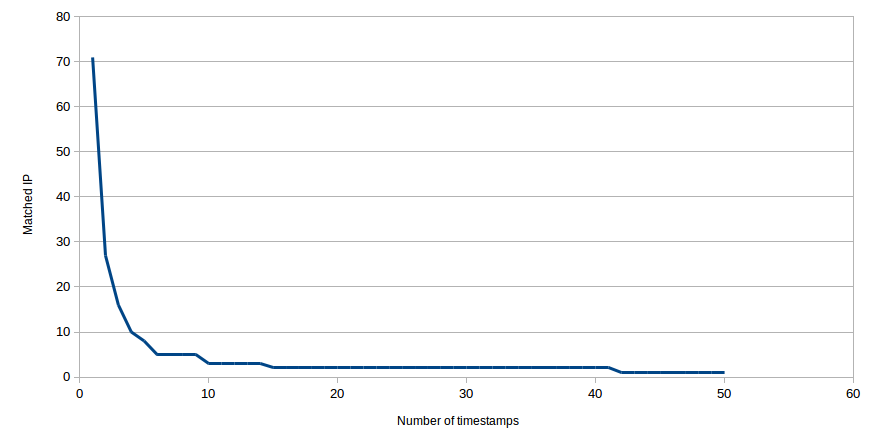
\includegraphics[width=180mm]{images/vk/online.png}
		\caption{The correlation between matched IP and number of timestamp}
	}
\end{figure}



